\documentclass[12pt]{article}
\usepackage[margin=0.75in]{geometry}
\geometry{a4paper}
\usepackage[T1]{fontenc} % Support Icelandic Characters
\usepackage[utf8]{inputenc} % Support Icelandic Characters
\usepackage{graphicx} % Support for including images
\usepackage{hyperref} % Support for hyperlinks
\usepackage{wrapfig}

\usepackage{algorithm}
\usepackage{algorithmicx}
\usepackage{listings}
\usepackage{color}
\usepackage{siunitx}

\usepackage[svgnames]{xcolor}

\usepackage{amsmath}
\usepackage{tikz}
\usetikzlibrary{arrows,automata}

\usepackage{tikz}
\usepackage{tikz-dependency}
\usepackage[spanish,es-noshorthands]{babel}

\usepackage[spanish]{babel}
\usepackage[latin1]{inputenc}
\usepackage[usenames]{color}

\definecolor{mGreen}{rgb}{0,0.6,0}
\definecolor{mGray}{rgb}{0.5,0.5,0.5}
\definecolor{mPurple}{rgb}{0.58,0,0.82}
\definecolor{backgroundColour}{rgb}{0.95,0.95,0.92}

\usepackage{xcolor}

\usepackage{listings}             % Include the listings-package
\lstdefinestyle{CStyle}{
    backgroundcolor=\color{backgroundColour},   
    commentstyle=\color{mGreen},
    keywordstyle=\color{blue},
    numberstyle=\tiny\color{mGray},
    stringstyle=\color{red},
    basicstyle=\footnotesize,
    breakatwhitespace=false,         
    breaklines=true,                 
    captionpos=b,                    
    keepspaces=true,                 
    numbers=left,                    
    numbersep=5pt,                  
    showspaces=false,                
    showstringspaces=false,
    showtabs=false,                  
    tabsize=2,
    language=C
}



%------------------------------------------------------------------
% TITLE
%------------------------------------------------------------------

\title{
\centerline{
    
\includegraphics[width=75mm]{unsa.png}}
    \vspace{0.5 cm}
        Teoría de la Computación - Laboratorio A
        \\
        \\
        \\
        \textbf{Práctica de Laboratorio #8} 
        \large  
        \\
        %SC-T-718-ATSR,Automatic Speech Recognition, 2019-1 
        %\\ 
        \small Universidad Nacional de San Agustín - Escuela Profesional de Ingeniería de Sistemas, Arequipa, Perú 
  }

\author{
    Carlos Alberto Mestas Escarcena
    \\
    \texttt{cmestas@unsa.edu.pe}
}

\date{Julio del 2020}

\begin{document}

\maketitle

El desarrollo de este informe se puede encontrar en el repositorio de \textcolor{blue}{
    \href{https://github.com/CarlosMestas/TC_A_9_Carlos_Mestas}{GitHub}}.
\\
\newline

\section{Ejercicio 1}

\begin{lstlisting}[language=bash,frame=single,style=CStyle,caption={lexico.l}]
%{
#include"sintactico.tab.h"
/*
externt yylval
*/
%}
numero [0-9]+
id [a-zA-Z]+
%%
{numero}            {yylval.atributos.valor = atoi(yytext);
                    yylval.atributos.tipo = "entero";   
                    return ENTERO;
                    }
{id}                {yylval.name = yytext; 
                    return ID;
                    }
"\n"                {return FINLINEA;}
"("                 {return PAR_IZQ;}
")"                 {return PAR_DER;}
"+"                 {return SUMA;}
"-"                 {return RESTA;}
"*"                 {return MULT;}
"/"                 {return DIV;}
"="                 {return IGUAL;}
" "                 ;
%%
int yywrap(){ return 0;}
\end{lstlisting}

\begin{lstlisting}[language=bash,frame=single,style=CStyle,caption={sintactico.y}]
%{
  #include <stdio.h>
  #include <string.h>
  #include <stdlib.h>
  #define YYDEBUG 1
  extern int yylex(void);
  extern char *yytext;
  void yyerror (char*);
%}

%union{
  struct var{
    char* tipo;
    int valor;
  } atributos;
  struct var2{
    char* tipo;
    int valor;
    char* nombre;
  } variable;
  char* name;
}

%token <name> ID
%token FINLINEA
%token <atributos> ENTERO
%token PAR_DER PAR_IZQ
%token IGUAL

%left SUMA RESTA
%left MULT DIV

%type <atributos> e
%type <variable> v
%type <name> i

%%
s: e FINLINEA {printf("= %d y es de tipo %s", $1.valor, $1.tipo);
              }
 | v FINLINEA {printf("La variable %s vale %d y es de tipo ... %s",$1.nombre,$1.valor, $1.tipo);
              }
;

v: i IGUAL e  {
                $$.tipo= $3.tipo;
                $$.valor = $3.valor;
                $$.nombre = $1;
              }
;
e: e SUMA e  {  $$.valor = $1.valor + $3.valor;
                $$.tipo= $1.tipo; 
             }
 | e RESTA e {  $$.valor = $1.valor - $3.valor;
                $$.tipo= $1.tipo; 
             }
 | e MULT e  {  $$.valor = $1.valor * $3.valor;
                $$.tipo= $1.tipo; 
             }
 | e DIV e   {
                if($3.valor == 0){
                  yyerror("No existe division entre 0");
                  exit(0);
                }
                else{
                  $$.valor = $1.valor / $3.valor;
                  $$.tipo= $1.tipo; 
                }  
             }                                           
 | ENTERO    {  $$.valor = $1.valor;
                $$.tipo = $1.tipo;
             } 
 ;
i: ID        {$$ = $1;}
 ; 
%%
void yyerror(char *s){
  printf("Error sintactico %s",s);
}

int main(int argc,char **argv){
  yydebug = 0;
  yyparse();
  return 0;
}
\end{lstlisting}
Comprobando de que el valor del divisor sea igual a cero, podemos decir que no se puede realizar la operación, se tiene un ejemplo de la ejecución:

\begin{figure}[h]
    \centering
    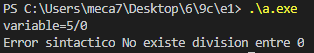
\includegraphics[width=0.5\textwidth]{images/Capture01A.PNG}
    \caption{Ejemplo de compilación}
\end{figure}

\clearpage
\newpage

\section{Ejercicio 2}

\begin{lstlisting}[language=bash,frame=single,style=CStyle,caption={lexico.l}]
%{
#include"sintactico.tab.h"
/*
externt yylval
*/
%}
digito [0-9]
numero {digito}+(\.{digito}+)?
id [a-zA-Z]+
%%
{numero}            {yylval.atributos.valor = atof(yytext);
                    yylval.atributos.tipo = "flotante";   
                    return FLOAT;
                    }
{id}                {yylval.name = yytext; 
                    return ID;
                    }
"\n"                {return FINLINEA;}
"("                 {return PAR_IZQ;}
")"                 {return PAR_DER;}
"+"                 {return SUMA;}
"-"                 {return RESTA;}
"*"                 {return MULT;}
"/"                 {return DIV;}
"="                 {return IGUAL;}
" "                 ;
%%
int yywrap(){ return 0;}
\end{lstlisting}

\begin{lstlisting}[language=bash,frame=single,style=CStyle,caption={sintactico.y}]
%{
  #include <stdio.h>
  #include <string.h>
  #include <stdlib.h>
  #define YYDEBUG 1
  extern int yylex(void);
  extern char *yytext;
  void yyerror (char*);
%}

%union{
  struct var{
    char* tipo;
    float valor;
  } atributos;
  struct var2{
    char* tipo;
    float valor;
    char* nombre;
  } variable;
  char* name;
}

%token <name> ID
%token FINLINEA
%token <atributos> FLOAT
%token PAR_DER PAR_IZQ
%token IGUAL

%left SUMA RESTA
%left MULT DIV

%type <atributos> e
%type <variable> v
%type <name> i

%%
s: e FINLINEA {printf("= %f y es de tipo %s", $1.valor, $1.tipo);
              }
 | v FINLINEA {printf("La variable %s vale %f y es de tipo ... %s",$1.nombre,$1.valor, $1.tipo);
              }
;

v: i IGUAL e  {
                $$.tipo= $3.tipo;
                $$.valor = $3.valor;
                $$.nombre = $1;
              }
;
e: e SUMA e  {  $$.valor = $1.valor + $3.valor;
                $$.tipo= $1.tipo; 
             }
 | e RESTA e {  $$.valor = $1.valor - $3.valor;
                $$.tipo= $1.tipo; 
             }
 | e MULT e  {  $$.valor = $1.valor * $3.valor;
                $$.tipo= $1.tipo; 
             }
 | e DIV e   {
                if($3.valor == 0){
                  yyerror("No existe division entre 0");
                  exit(0);
                }
                else{
                  $$.valor = $1.valor / $3.valor;
                  $$.tipo= $1.tipo; 
                }  
             }                                           
 | FLOAT    {  $$.valor = $1.valor;
                $$.tipo = $1.tipo;
             } 
 ;
i: ID        {$$ = $1;}
 ; 
%%
void yyerror(char *s){
  printf("Error sintactico %s",s);
}
\end{lstlisting}
En comparación al ejercicio anterior se realizó unos pequeños cambios, en el léxico, para que de esta forma se puedan ingresar números reales, así como un cambio de $atoi$ por $atof$ para que se pueda convertir a un flotante, se cambió también el valor del token a \textbf{FLOAT}, para el sintáctico, se cambió un valor del struc de $int$ a $float$.

\clearpage
\newpage

\begin{figure}[h]
    \centering
    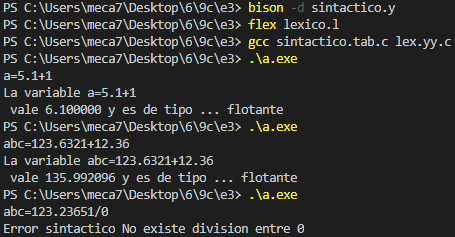
\includegraphics[width=0.5\textwidth]{images/Capture02A.PNG}
    \caption{Ejemplo de compilación}
\end{figure}

\section{Ejercicio 3}

\begin{lstlisting}[language=bash,frame=single,style=CStyle,caption={lexico.l}]
%{
#include"sintactico.tab.h"
/*
externt yylval
*/
%}
digito [0-9]
numeroInt   {digito}+
numeroFloat {digito}+(\.{digito}+)?
id [a-zA-Z]+
%%
{numeroInt}         {yylval.atributos2.valor = atoi(yytext);
                    yylval.atributos2.tipo = "entero";   
                    return ENTERO;
                    }
{numeroFloat}       {yylval.atributos.valor = atof(yytext);
                    yylval.atributos.tipo = "flotante";   
                    return FLOAT;
                    }
{id}                {yylval.name = yytext; 
                    return ID;
                    }
"\n"                {return FINLINEA;}
"("                 {return PAR_IZQ;}
")"                 {return PAR_DER;}
"+"                 {return SUMA;}
"-"                 {return RESTA;}
"*"                 {return MULT;}
"/"                 {return DIV;}
"="                 {return IGUAL;}
" "                 ;
%%
int yywrap(){ return 0;}
\end{lstlisting}

\begin{lstlisting}[language=bash,frame=single,style=CStyle,caption={sintactico.y}]
%{
  #include <stdio.h>
  #include <string.h>
  #include <stdlib.h>
  #define YYDEBUG 1
  extern int yylex(void);
  extern char *yytext;
  void yyerror (char*);
%}

%union{
  struct var{
    char* tipo;
    float valor;
  } atributos;
  struct var2{
    char* tipo;
    float valor;
    char* nombre;
  } variable;
  struct var3{
    char* tipo;
    int valor;
  } atributos2;
  struct var4{
    char* tipo;
    int valor;
    char* nombre;
  } variable2;
  char* name;
}

%token <name> ID
%token FINLINEA
%token <atributos> FLOAT
%token <atributos2> ENTERO
%token PAR_DER PAR_IZQ
%token IGUAL

%left SUMA RESTA
%left MULT DIV

%type <atributos> e
%type <variable> v
%type <atributos2> e2
%type <variable2> v2
%type <name> i

%%
s: e  FINLINEA {printf("= %f y es de tipo %s", $1.valor, $1.tipo);
               }
 | v  FINLINEA {printf("La variable %s vale %f y es de tipo ... %s",$1.nombre,$1.valor, $1.tipo);
               }
 | e2 FINLINEA {printf("= %d y es de tipo %s", $1.valor, $1.tipo);
               }
 | v2 FINLINEA {printf("La variable %s vale %d y es de tipo ... %s",$1.nombre,$1.valor, $1.tipo);
               }
;

v: i IGUAL e  {
                $$.tipo= $3.tipo;
                $$.valor = $3.valor;
                $$.nombre = $1;
              }
;
v2: i IGUAL e2  {
                  $$.tipo= $3.tipo;
                  $$.valor = $3.valor;
                  $$.nombre = $1;
                }
;
e: e SUMA e     {  $$.valor = $1.valor + $3.valor;
                   $$.tipo= $1.tipo; 
                }
 | e RESTA e    {  $$.valor = $1.valor - $3.valor;
                   $$.tipo= $1.tipo; 
                }
 | e SUMA e2    {  $$.valor = $1.valor + $3.valor;
                   $$.tipo= $1.tipo; 
                }  
 | e2 SUMA e    {  $$.valor = $1.valor + $3.valor;
                   $$.tipo= $3.tipo; 
                }                   
 | e RESTA e2    {  $$.valor = $1.valor - $3.valor;
                    $$.tipo= $1.tipo; 
                 }  
 | e2 RESTA e    {  $$.valor = $1.valor - $3.valor;
                    $$.tipo= $3.tipo; 
                 }                                                                                  
 | FLOAT        {  $$.valor = $1.valor;
                   $$.tipo = $1.tipo;
                }             
             
 ;
e2: e2 SUMA e2  {  $$.valor = $1.valor + $3.valor;
                   $$.tipo= $1.tipo; 
                }
  | e2 RESTA e2 {  $$.valor = $1.valor - $3.valor;
                   $$.tipo= $1.tipo; 
                }
  | ENTERO      {  $$.valor = $1.valor;
                   $$.tipo = $1.tipo;
                } 
             
 ;
i: ID        {$$ = $1;}
 ; 
%%
void yyerror(char *s){
  printf("Error sintactico %s",s);
}

int main(int argc,char **argv){
  yydebug = 0;
  yyparse();
  return 0;
}
\end{lstlisting}
En este ejemplo podemos ver una unión de los dos ejemplos anteriores en el léxico, ya que ahora retornaremos dos tokens diferentes \textbf{ENTERO y FLOAT}, así como también relacionarlos a los struct del sintáctico, en este caso también en el caso de tener una suma de un valor entero con un real o un valor real con un entero, al final el resultado será real, por ello tanto en la suma como en la resta los asociamos al no terminal que opera con los flotantes, así como al asignar el tipo de variable, le asignamos el tipo de variable flotante.

\begin{figure}[h]
    \centering
    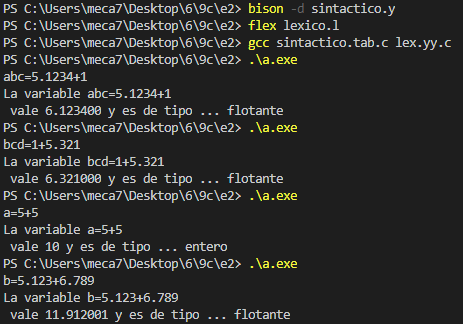
\includegraphics[width=0.8\textwidth]{images/Capture03A.PNG}
    \caption{Ejemplo de compilación}
\end{figure}

\end{document}